\chapter{Authenticating {kNN} Queries in Distributed Environment}\label{chap:knn}

In this chapter, we investigate the problem of authenticating {kNN} queries in distributed environment.

\section{Problem Formulation}\label{sec:knn:problem}

There are three parties in our system: the DO, the third-party distributed SP, and the client. The DO builds the ADS and signs the ADS to ensure the integrity of the data. The ADS and the signature are then sent to the SP\@. The distributed SP provides the service of storage and query processing. Since the SP is configured in a distributed environment, it consists of several types of nodes: $Master$, $Slave$, and $Reducer$. The $Master$ node in the SP is mainly responsible for dispatching jobs to the corresponding slaves. The $Slave$ nodes are the workers, which process the actual queries. The $Reducer$ consolidates all the partial results as well as the VOs computed by the $Slaves$ and sends them to the client. Finally, the client can verify the soundness and completeness of the results by using the VO, the DO's public key, and the root signature sent by the SP\@.

\textbf{Threat Model.}
In this system, we consider the DO as the trusted party. The SP is untrusted and can return incorrect results. Given the whole dataset $D$, the client's query point $q$, and the parameter $k$, the SP returns several results. If the result number does not match the value $k$, the client can find that some results are missing. Suppose $R_{k}=\{r_{1},r_{2},\dots,r_{k}\}$ are the $k$ true kNN results. The SP can
\begin{inlineenum}
\item return a point $p$ and $p \notin D$;
\item return a point $p \in D$ but $dist(q,p) > dist(q,r_{k})$, where $dist(\cdot,\cdot)$ denotes the Euclidean distance.
\end{inlineenum}
The first and second cases violate the soundness and completeness conditions, respectively.

The system's performance can be measured in these metrics:
\begin{inlineenum}
\item ADS construction time;
\item query processing cost;
\item client's verification time; and
\item VO size.
\end{inlineenum}
We assume that there is no data update in this system. Therefore, the ADS construction is a one-off operation by the DO and the cost can be amortized by the queries. The VO size can influence the communication overhead between the SP and the client as well as the time of client's verification. Therefore, the VO size should be minimized.

\section{Preliminaries}\label{sec:knn:prelim}

\subsection{Cryptographic Primitives}

In our solution, two cryptographic primitives are used, namely hash function and digital signature.

\textbf{Hash Function}: A one-way hash function $H(\cdot)$ transforms an arbitrary message $m$ to a fixed-length digest $H(m)$. One-way indicates that given a message $m$, the computation of $H(m)$ is easy. However, to get $m$ from $H(m)$ is computationally infeasible. In this chapter, we use SHA-1 as the hash function, which maps a given message to a 160-bit digest.

\textbf{Digital Signature}: The asymmetric signature is used to verify the integrity of the data. The DO keeps a secret key and publishes the corresponding public key to the verifier. The DO signs the data using the secret key and the verifier can decrypt the signature using the public key and verify the integrity of the data. RSA is one of the popular asymmetric signature algorithms.

\subsection{Spatial Authenticated Data Structure}

MR-tree~\cite{10.1007/s00778-008-0113-2}, which is the combination of the R-tree and the Merkle Hash tree~\cite{10.1007/0-387-34805-0_21}, is often used to process authenticated spatial queries. Each leaf node stores the pointers pointing to the data points and the hash value of the binary concatenation of the data points. The hash value of an internal node is computed by hashing the concatenation of each child node's MBR and hash value. We give an example based on \Cref{fig:knn:local-mrtree}, which depicts the data points and their corresponding MR-tree. The leaf node $N_{3}$'s hash value is $H(a|b|c)$, where `$|$' represents the binary concatenation. The non-leaf node's hash value $H(N_{1})=H(N_{3}|H(N_{3})|N_{4}|H(N_{4}))$. Here $N_{3}, N_{4}$ represent the MBR of node $N_{3}$ and $N_{4}$, respectively. We only show three hash values in \Cref{fig:knn:local-mrtree} and other hash values are computed similarly.

\begin{figure}[t]
  \centering
  \begin{subfigure}[b]{.35\linewidth}
    \centering
    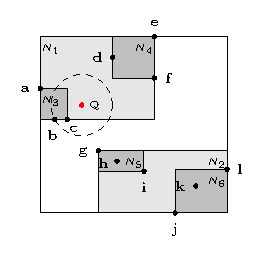
\includegraphics[width=\linewidth]{figs/knn/local-mrtree-data.pdf}
    \caption{Data}\label{fig:knn:local-mrtree:data}
  \end{subfigure}~%
  \begin{subfigure}[b]{.65\linewidth}
    \centering
    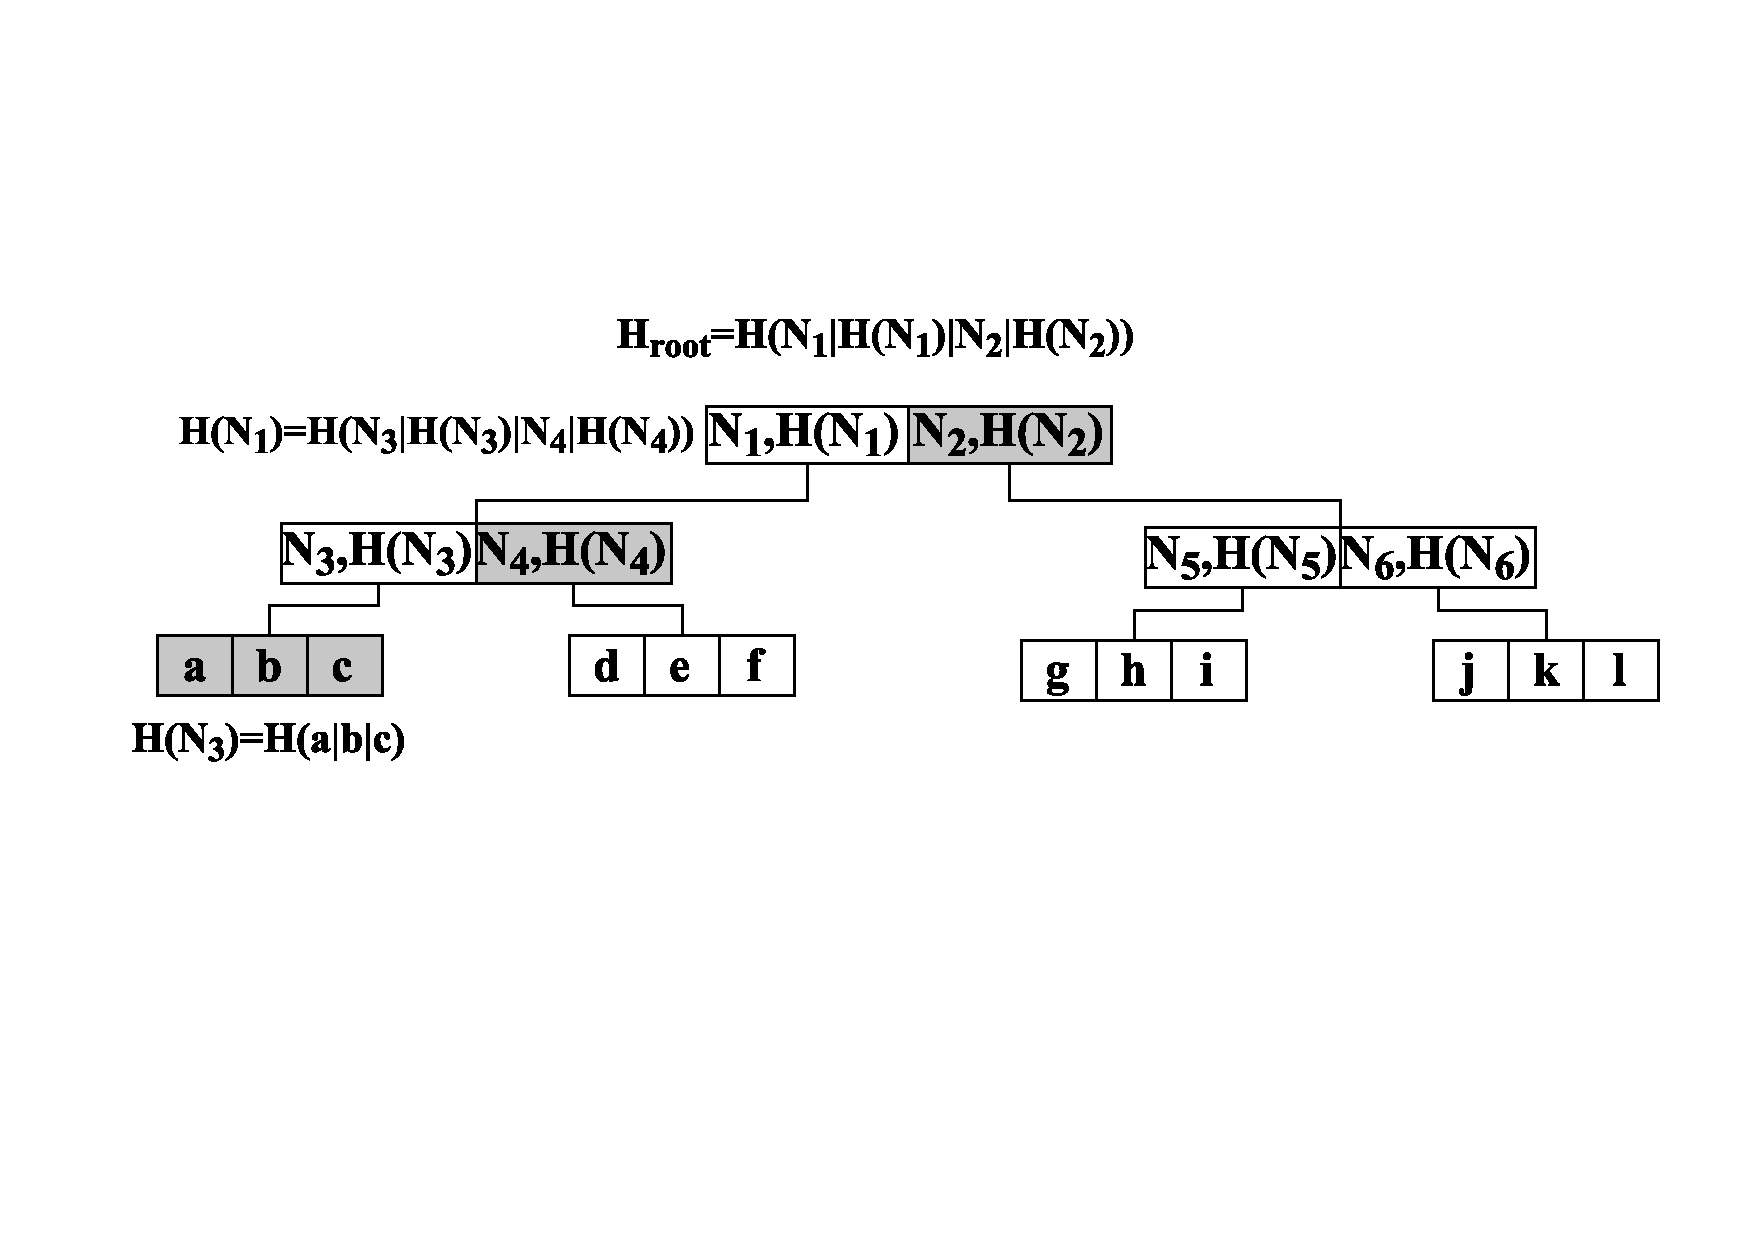
\includegraphics[width=\linewidth]{figs/knn/local-mrtree-tree.pdf}
    \caption{Index}\label{fig:knn:local-mrtree:tree}
  \end{subfigure}
  \caption{Local Authenticated {kNN} Processing}\label{fig:knn:local-mrtree}
\end{figure}

\subsection{Local Authenticated kNN Processing}
There are mainly two different methods of authenticated kNN processing based on the MR-tree. The algorithm proposed by \citeauthor{10.1007/s00778-008-0113-2}~\cite{10.1007/s00778-008-0113-2} mainly focuses on the authenticated range query and transforms the kNN query to a range query. The method separates the generation of the results and the VO\@. It first retrieves kNN results by using any kNN search method. Based on the $k$ results, we can draw a circle centered at the query point $q$ with the radius of the distance between $q$ and the $k^{th}$ result. Then, the authenticated range query is executed to generate the VO set. Another method is to generate the results and the VO set together while traversing the whole MR-tree. \citeauthor{10.1007/978-3-319-18120-2_33}~\cite{10.1007/978-3-319-18120-2_33} proposed the authentication of top-$k$ spatial keyword queries and we can transform this query to the authenticated kNN query easily. \Cref{alg:knn:knn} shows the procedure of generating the VO and results altogether.

\begin{algorithm}[t]
    \caption{Local Authenticated kNN Query}\label{alg:knn:knn}
    \KwIn{$k$, Point $q$, Root of MR-tree $\mathcal{T}_R$}
    \KwOut{Result set $RS$, Verification object $VO$}
    $RS \gets \emptyset$; $counter \gets 0$\;
    $VO \gets (\textrm{`['}, \mathcal{T}_R, \mathcal{T}_R.hash, \textrm{`]'})$\; % chktex 9
    Initialize priority queue $PQ$ and enqueue $\mathcal{T}_R$\;
    \While{$counter < k \land PQ \neq \emptyset$}{%
      $object \gets dequeue(PQ)$\;
      \eIf{$object$ is an MBR $R_i$}{%
        Enqueue each $R_{j}$ or $O_{j}$ in $R_{i}$'s child node into $PQ$\;
        Replace $R_{i}, R_{i}.hash$ with `[', each $R_{j}$, $R_{j}.hash$ (or $O_{j}$) in $R_{i}$'s child node, and `]' in $VO$\;
      }{%
        $RS \gets RS + \{object\}$\;
        $counter \gets counter + 1$\;
      }
    }
    \Return{$\langle RS, VO \rangle$}\;
\end{algorithm}

The algorithm traverses the MR-tree in a best first search manner~\cite{10.1145/320248.320255}. We maintain a priority queue $PQ$. In the while loop, the current nearest object to the point $q$ is dequeued from the priority queue $PQ$. If the object is a node rather than a data point, each of its child node $R_{j}$ will be enqueued to the $PQ$. Otherwise, the object is added to the result set because it is a point. The while loop terminates until $k$ results are collected or the $PQ$ is empty. The VO set changes along with the expansion of the object. The sign marks `[' and `]' are used to decide the scope of entries in a node and they can help the client reconstruct the root hash value. The VO set is initialized with `[', MR-tree root $\mathcal{T}_R$, $\mathcal{T}_R.hash$, and `]'. When the object is dequeued from the $PQ$, we replace $R_{i}$, $R_{i}.hash$ with `[', each $R_{j}$ and $R_{j}.hash$ (or $O_{j}$) in $R_{i}$'s child node, and `]'.

We give an example of the local authenticated kNN processing using \Cref{fig:knn:local-mrtree}. Assume that $k=2$ and the red point $Q$ is the query point. At first, the $PQ$ contains $N_{root}$ and the $VO$ is [$N_{root}, H_{root}$]. They will then be expanded to $N_1, N_2$ and [[$N_{1}$,$H(N_{1})$], [$N_{2}$,$H(N_{2})$]] respectively. Next, $N_{1}$ is removed and $N_{3}$, $N_{4}$ are added into the $PQ$. The $VO$ changes to [[[$N_{3}$, $H(N_{3})$], [$N_{4}$, $H(N_{4})$]], [$N_{2}$, $H(N_{2})$]]. Finally, points $c$ and $b$ are computed as the results and the $VO$ updates to [[[$a$,$b$,$c$], [$N_{4}$,$H(N_{4})$]], [$N_{2}$, $H(N_{2})$]]. The grey nodes in \Cref{fig:knn:local-mrtree:tree} are included in the $VO$. We omit the client verification part here as we will illustrate the verification for the distributed kNN authentication in \Cref{sec:knn:client-verification}.

\section{Distributed {kNN} Authentication}\label{sec:knn:distributed-knn}

\subsection{Distributed MR-Tree}

\begin{figure}[t]
  \centering
  \begin{subfigure}[b]{.35\linewidth}
    \centering
    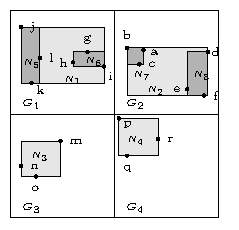
\includegraphics[width=\linewidth]{figs/knn/distributed-mrtree-data.pdf}
    \caption{Data}\label{fig:knn:distributed-mrtree:data}
  \end{subfigure}~%
  \begin{subfigure}[b]{.65\linewidth}
    \centering
    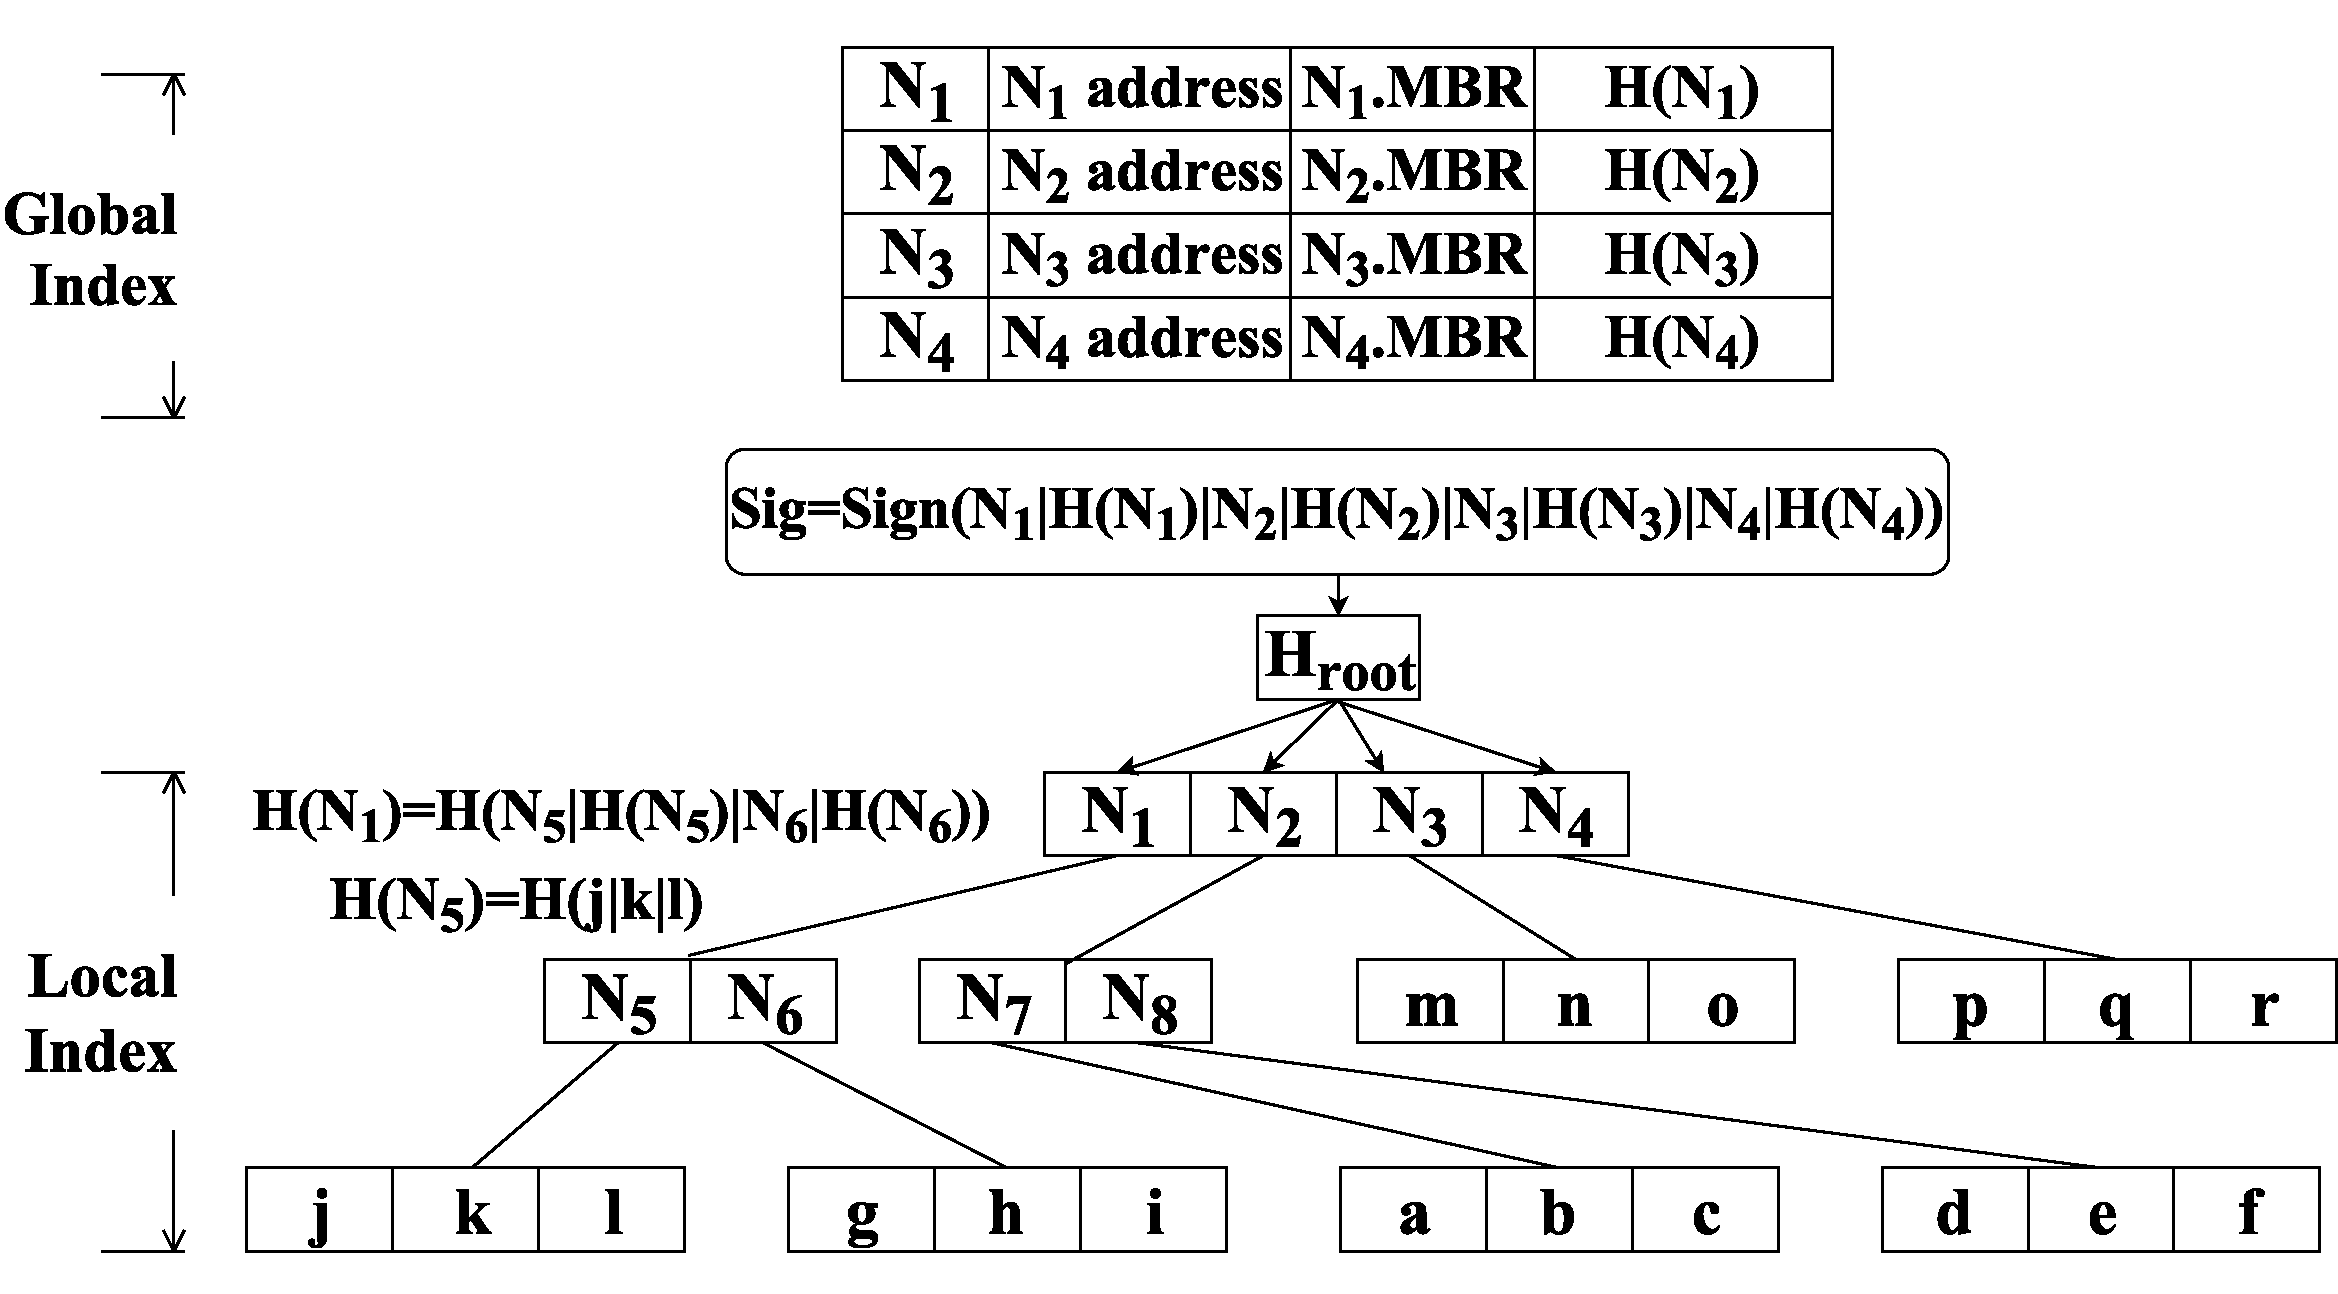
\includegraphics[width=\linewidth]{figs/knn/distributed-mrtree-tree.pdf}
    \caption{Index}\label{fig:knn:distributed-mrtree:tree}
  \end{subfigure}
  \caption{Distributed MR-tree}\label{fig:knn:distributed-mrtree}
\end{figure}

To adapt the MR-tree index structure to the distributed environment, the index structure has two layers: the local index and the global index. The DO first employs the Grid partition or the Sort-Tile-Recursive~\cite{10.1109/ICDE.1997.582015} method to partition the entire dataset into several splits. These methods guarantee that there is no overlap between any two partitions' minimum bounding rectangles (MBRs). Thanks to this non-overlapping characteristic, only a few partitions are used to process the kNN query, which saves the computation resources. The local indexes are constructed using the data points in each partition. The global index is then constructed, and it contains each local MR-tree's root MBR and, root hash value, and the pointers towards each local index. After the construction of the index structure, the DO signs the root node of the global index using the private key. Then, the signature and the entire index will be sent to the SP\@. The $Master$ of the SP is responsible for dispatching the local indexes to the $Slaves$ according to the current workload of the distributed system. Since the global index is small, it will be stored in the main memory of all the nodes, which can speed up the kNN query processing. \Cref{fig:knn:distributed-mrtree:data} shows the four partitions using the Grid partition method. \Cref{fig:knn:distributed-mrtree:tree} depicts the entire structure of distributed MR-tree. In each partition, the data points are used to build a local MR-tree. We use $N_{1}$, $N_{2}$, $N_{3}$ and $N_{4}$ to represent the four local indexes. The global index is a directory table and can prune the search space.

